\section{Introduction}

\begin{itemize}

\item What is the subject of the study? Describe the
economic/econometric problem.

-> Implementation of Cancer Gene Panels & Variant Calling Algorithms

\item What is the purpose of the study (working hypothesis)?

-> Check whether one of them is better than the others.
-> Study effect of FFPE

\item What do we already know about the subject (literature
review)? Use citations: { \cite{mutect:2013} shows that...
Alternative Forms of the Wald test are considered
\citep{Breusch&Schmidt:88}.}

\item What is the innovation of the study?

-> relatively rare technique in diagnostics, but has many advantages

\item Provide an overview of your results.


\end{itemize}

Cancer is a major public health problem worldwide and one of the leading death
causes. In 2012, there were an estimated 14.1 million new cancer cases with
estimated  8.2 million cancer deaths {\cite{cancer_stats_worldwide:2012}}. Lung
cancer is the most common cancer, both in terms of new cases (1.8 million) and
deaths (1.6 million). Breast  cancer is the second most common cancer (1.7
million cases) but only ranks 5th as cause of death (522,000 deaths). Colorectal
cancer (1.4 million cases; 694,000 deaths), prostate cancer (1.1 million cases;
307,000 deaths), stomach cancer (951,000 cases; 723,000 deaths) and liver cancer
(782,000 cases; 723,000 deaths) are following.

In Luxembourg, there were 1164 death cases caused by cancer in 2014, accounting
for 30.6\%  of the number of deaths. Cancer is thereby the second most common
death cause in Luxembourg, ranging behind cardiovascular diseases (1189 deaths;
31.3\%). Amongst these cancer deaths, cancers of the digestive organs (340
deaths) and of the respiratory organs (272 deaths) were the most frequent ones.
{\cite{cancer_stats:2012}}.

(Considerable effort is made by the research
community to understand the underlying causes of cancer and its progression, but
death rate related to cancer remains high. In Luxembourg, the death rate did not
significantly drop from 1998 to 2014.)

In recent years, more targeted drugs. personalized medicine.

Next-Generation Sequencing (NGS) is a powerful method to analyze RNA or DNA
molecules. Improved protocols and methods have been developed in recent years
that allow to implement NGS for a variety of applications in both research and
diagnostics. NGS is still hard to implement and is mainly used in research. Only
a few laboratories are using this technique as a diagnostic technique.The SGMB
is building expertise in NGS and is implementing targeted NGS in its molecular
pathology laboratory. This implementation aims at gaining deep insights into the
underlying causes of solid tumors and in guiding targeted cancer therapy.

The goal of this master's thesis was to compare commercially available cancer
gene panels on samples of solid tumor patients by several parameters and by
their ability to detect variants, which have previously been detected in the
routine mutation detection workflow in the laboratory. As a second part, several
freely available variant calling algorithms were compared for their potential
implementation in the custom in-house variant detection bioinformatic pipeline.

\subsection{EGFR Signaling in Cancer}

Bla {\cite{targeting_egfr:2012}}

Describe pathway

\begin{figure}[ht]
  \begin{center}
    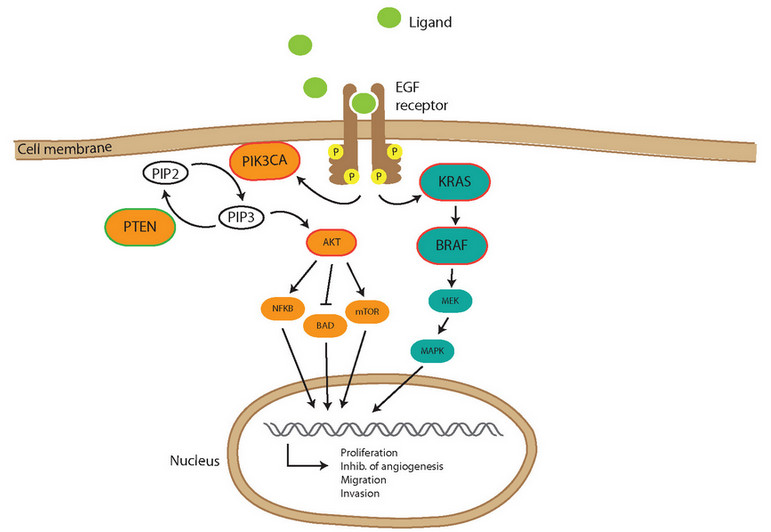
\includegraphics[scale=1,angle=0]{egfr_signaling.png}
    \caption{Schematic representation of the EGFR signaling cascade {\cite{targeting_egfr:2012}}}
    \label{Fig:egfr_signaling}
  \end{center}
\end{figure}

Common mutations in this pathway

EGFR-targeted drugs:
bevacizumab, cetuximab, panitumumab, ...

\subsection{Targeted Sequencing and Target Enrichment Methods}

Sanger Sequencing

Human Genome Project

Benchtop sequencing devices: more labs can now do sequencing as it becomes faster
& cheaper & more reliable. 

More & more databases describing SNPs & known pathogenic hotspots

targeted sequencing as um kommen, cost-effective & fast & high-coverage

Bla {\cite{enrichment_methods:2011}}

Hybrid capture

Selective circularization

PCR amplification

\subsection{Sequencing Chemistries}

IonTorrent, etc

\subsubsection{Illumina MiSeq}

Picture

\subsection{NGS Data Analysis}

GATK best practices

\subsection{Practical Implications in the Laboratory}

FFPE : more details

Chemical fixatives are used to preserve tissue from degradation, and to maintain
the structure of the cell and of sub-cellular components such as cell organelles
(e.g., nucleus, endoplasmic reticulum, mitochondria). The most common fixative
for light microscopy is 10% neutral buffered formalin (4% formaldehyde in
phosphate buffered saline).

These fixatives preserve tissues or cells mainly by irreversibly cross-linking
proteins. The main action of these aldehyde fixatives is to cross-link amino
groups in proteins through the formation of methylene bridges (-CH2-), in the
case of formaldehyde.

This process, while preserving the structural integrity of the cells and tissue
can damage the biological functionality of proteins, particularly enzymes, and
can also denature them to a certain extent. This can be detrimental to certain
histological techniques.

Formalin fixation leads to degradation of mRNA, miRNA and DNA in tissues.
However, extraction, amplification and analysis of these nucleic acids from
formalin-fixed, paraffin-embedded tissues is possible using appropriate
protocols.

The aim of Tissue Processing is to remove water from tissues and replace with a
medium that solidifies to allow thin sections to be cut. Biological tissue must
be supported in a hard matrix to allow sufficiently thin sections to be cut,
typically 5 μm (micrometres; 1000 micrometres = 1 mm) thick for light microscopy.

Since it is immiscible with water, the main constituent of biological tissue,
water must first be removed in the process of dehydration. Samples are
transferred through baths of progressively more concentrated ethanol to remove
the water. This is followed by a hydrophobic clearing agent (such as xylene) to
remove the alcohol, and finally molten paraffin wax, the infiltration agent,
which replaces the xylene. Paraffin wax does not provide a sufficiently hard
matrix for cutting very thin sections for electron microscopy. Instead, resins
are used. Epoxy resins are the most commonly employed embedding media, but
acrylic resins are also used, particularly where immunohistochemistry is
required. Thicker sections (0.35μm to 5μm) of resin-embedded tissue can also be
cut for light microscopy. Again, the immiscibility of most epoxy and acrylic
resins with water necessitates the use of dehydration, usually with ethanol.

After the tissues have been dehydrated, cleared, and infiltrated with the
embedding material, they are ready for external embedding. During this process
the tissue samples are placed into molds along with liquid embedding material
(such as agar, gelatine, or wax) which is then hardened. This is achieved by
cooling in the case of paraffin wax and heating (curing) in the case of the
epoxy resins. The acrylic resins are polymerised by heat, ultraviolet light, or
chemical catalysts. The hardened blocks containing the tissue samples are then
ready to be sectioned.

Because Formalin-fixed, paraffin-embedded (FFPE) tissues may be stored
indefinitely at room temperature, and nucleic acids (both DNA and RNA) may be
recovered from them decades after fixation, FFPE tissues are an important
resource for historical studies in medicine.

For light microscopy, a steel knife mounted in a microtome is used to cut
4-micrometer-thick tissue sections which are mounted on a glass microscope
slide. For transmission electron microscopy, a diamond knife mounted in an
ultramicrotome is used to cut 50-nanometer-thick tissue sections which are
mounted on a 3-millimeter-diameter copper grid. Then the mounted sections are
treated with the appropriate stain.

quantitation

ffpe quality control necessary. FFPE are degraded. More C>T

Target enrichment methods hun och vlt en effekt

choice vum sequencer, different error rates, different yield, analysis time.

choice vun den bioinformatic tools. t'gin der vill, vir- an nodeeler. zB variant
calling algorithms: most are for haplotypes and not for somatic variants. many
need matched tumor-normal samples, which we here in the lab do not have, only have
tumor dna. after variant calling, they have to be annotated for their clinical
relevance and potential actionability.

problem: many variants may be found, some of them may be
harmless germline SNPs, many variants may be causative of cancer, but are not actionable.

time sample-to-result

how to report? all results or only those that are known to be actionable.

\subsection{Aims of the Thesis}
Targeted NGS is still not widely used in diagnostics laboratories. The SGMB of the LNS
is planning to build expertise with the aim to adopt NGS routinely in the laboratory,
mainly in the context of diagnosis and therapy of cancer patients in Luxembourg.

The aim of this thesis project was to test commercially available cancer gene panels,
e.g. Illumina Trusight Tumor 15 and Agilent Haloplex HS ClearSeq Cancer, for their
potential use in the routine workflow of the laboratory. Several samples of cancer
patients were prepared with both kits and were sequenced on the Illumina MiSeq device.
Both kits vary in their sequencing library preparation principles: Illumina's tst15
uses the multiplex PCR approach while Agilent's Haloplex Enrichment System uses
enzymatic DNA restriction followed by probe capture.

NGS data were analyzed with the respective recommended pipelines and a custom in-house
pipeline.

Finally, several freely available variant calling algorithms were tested for their
potential implementation in the custom in-house variant discovery bioinformatic
pipeline.
